\documentclass[12pt,twoside]{article}
\usepackage[russian,english]{babel}
\usepackage[utf8]{inputenc}
\usepackage{abstract}
\usepackage{amsmath,amssymb,mathrsfs,mathtext,amsthm}
\usepackage{a4wide}
\usepackage[T2A]{fontenc}
\usepackage{subfig}
\usepackage{url}
\usepackage[usenames]{color}
\usepackage{colortbl}

\newcommand{\hdir}{.}
\usepackage{hyperref}       % clickable links
\usepackage{lineno}
\usepackage{graphicx,multicol}
\usepackage{epstopdf}
\usepackage{cite}
\usepackage{amsmath,amssymb,mathrsfs,mathtext}
\usepackage{tikz}
\usetikzlibrary{shapes,arrows,shadows}
\newtheorem{theorem}{Theorem}
\newtheorem{statement}{Statement}
\usepackage{algorithm}
\usepackage[noend]{algcompatible}

\usepackage{caption}

%\renewcommand{\baselinestretch}{1.4}


\newcommand{\bx}{\mathbf{x}}
\newcommand{\by}{\mathbf{y}}
\newcommand{\bw}{\mathbf{w}}
\newcommand{\ba}{\mathbf{a}}
\newcommand{\bb}{\mathbf{b}}
\newcommand{\bY}{\mathbf{Y}}
\newcommand{\bX}{\mathbf{X}}
\newcommand{\bu}{\mathbf{u}}
\newcommand{\bt}{\mathbf{t}}
\newcommand{\bp}{\mathbf{p}}
\newcommand{\bq}{\mathbf{q}}
\newcommand{\bc}{\mathbf{c}}
\newcommand{\bP}{\mathbf{P}}
\newcommand{\bT}{\mathbf{T}}
\newcommand{\bB}{\mathbf{B}}
\newcommand{\bQ}{\mathbf{Q}}
\newcommand{\bC}{\mathbf{C}}
\newcommand{\bE}{\mathbf{E}}
\newcommand{\bF}{\mathbf{F}}
\newcommand{\bU}{\mathbf{U}}
\newcommand{\bW}{\mathbf{W}}
\newcommand{\bbR}{\mathbb{R}}
\newcommand{\cA}{\mathcal{A}}
\newcommand{\bchi}{\boldsymbol{\chi}}
\newcommand{\bnu}{\boldsymbol{\nu}}
\newcommand{\bmu}{\boldsymbol{\mu}}
\newcommand{\btheta}{\boldsymbol{\theta}}
\newcommand{\bTheta}{\boldsymbol{\Theta}}
\newcommand{\bOne}{\boldsymbol{1}}
\newcommand{\bZero}{\boldsymbol{0}}
\newcommand{\argmin}{\mathop{\arg \min}\limits}
\newcommand{\argmax}{\mathop{\arg \max}\limits}

\newcommand\undermat[2]{%
	\makebox[0pt][l]{$\smash{\underbrace{\phantom{%
					\begin{matrix}#2\end{matrix}}}_{\text{$#1$}}}$}#2}


\begin{document}

\linenumbers
%%%%%%%%%%%%%%%%%%%%%%%%%%%%%%%%%%%%%%%%%%%%%%%%
\section{Problem statement}
%%%%%%%%%%%%%%%%%%%%%%%%%%%%%%%%%%%%%%%%%%%%%%%%

The goal is to forecast a dependent variable $\by \in \bbR^r$ with $r$ targets from an independent input object $\bx \in \bbR^n$ with $n$ features.
We assume there is a linear dependence 
\begin{equation}
	\by = \bTheta \bx+ \boldsymbol{\varepsilon}
	\label{eq:model}
\end{equation}
between the objects $\bx$ and the target variable $\by$,
where $\bTheta \in \bbR^{r \times n}$ is the matrix of model parameters, $\boldsymbol{\varepsilon} \in \bbR^{r}$ is the residual vector.
The task is to find the matrix of the model parameters $\bTheta$ given a dataset $\left( \bX, \bY \right)$, where $\bX \in \bbR^{m \times n}$ is a design matrix, $\bY \in \bbR^{m \times r}$ is a target matrix
\[
	\bX = [\bx_1, \dots, \bx_m]^T =  [\bchi_1, \dots, \bchi_n]; \quad \bY = [\by_1, \dots, \by_m]^T =  [\bnu_1, \dots, \bnu_r].
\]
The columns~$\bchi_j$ of the matrix~$\bX$ respond to object features. 
The examples of how to construct the dataset for a particular application task are described in Section \hyperref[sec:exper]{Computational experiment}.

The optimal parameters are determined by minimization of an error function. 
Define the quadratic error function:
\begin{equation}
	S(\bTheta | \bX, \bY) = {\left\| \underset{m \times r}{\mathbf{Y}}  - \underset{m \times n}{\bX} \cdot \underset{r \times n}{\bTheta}^T \right\| }_2^2 \rightarrow\min_{\bTheta}.
\label{eq:error_function}
\end{equation}
 
 The solution of the problem~\eqref{eq:error_function} is given by
 \[
 	\bTheta = (\bX^T \bX)^{-1} \bX^T \bY.
 \]
 
 The linear dependent columns of the matrix $\bX$ leads to an instable solution for the optimization problem~\eqref{eq:error_function}. 
 If there is a vector $\boldsymbol{\alpha} \neq 0$ such that $\bX \boldsymbol{\alpha}= 0$, then adding the vector~$\boldsymbol{\alpha}$ to any column of the matrix~$\bTheta$ does not change the error function $S(\bTheta | \bX, \bY)$.
 In this case the matrix $\bX^T \bX$ is not invertible.
 To avoid the strong linear dependence, feature selection and dimensionality reduction techniques are used.
 
 %%%%%%%%%%%%%%%%%%%%%%%%%%%%%%%%%%%%%%%%%%%%%%%%
 \section{Feature selection}
 %%%%%%%%%%%%%%%%%%%%%%%%%%%%%%%%%%%%%%%%%%%%%%%%
 The feature selection goal is to find the index set~$\cA = \{1, \dots, n\}$ of the matrix $\bX$ columns. To select the set~$\cA$ among all possible $2^n - 1$ subsets, introduce the feature selection quality criteria
\begin{equation}
	\cA = \argmax_{\cA' \subseteq \{1, \dots, n\}} Q(\cA' | \bX, \bY).
	\label{eq:subset_selection}
\end{equation}

Once the solution~$\cA$ for the problem~\eqref{eq:subset_selection} is known, the problem~\eqref{eq:error_function} becomes
\begin{equation}
S(\bTheta_{\cA} | \bX_{\cA}, \bY) = {\left\| \mathbf{Y} - \bX_{\cA}\bTheta^T_{\cA} \right\| }_2^2 \rightarrow\min_{\bTheta_{\cA}},
\end{equation}
where the subscript~$\cA$ indicates columns with indices from the set~$\cA$.

\subsection{Quadratic Programming Feature Selection}
One of the approach to the feature selection is to maximize feature relevances and minimize pairwise feature redundancy.
The QPFS algorithm selects non-correlated features, which are relevant to the target vector~$\bnu$ for the linear regression problem ($r=1$)
\begin{equation*}
	\| \bnu - \bX \btheta\|_2^2 \rightarrow\min_{\btheta \in \bbR^{n}}.
\end{equation*}
Introduce two functions: $\text{Sim}(\bX)$ and $\text{Rel}(\bX, \bnu)$. 
The $\text{Sim}(\bX)$ measures the redundancy between features, the $\text{Rel}(\bX, \bnu)$ contains relevances between each feature and the target vector~$\bnu$. 
We want to minimize the function Sim and maximize the Rel simultaneously.

QPFS offers the explicit way to construct the functions Sim and Rel. 
The method minimizes the following functional
\begin{equation}
	(1 - \alpha) \cdot \underbrace{\ba^T \bQ \ba}_{\text{Sim}} - \alpha \cdot \underbrace{\vphantom{()} \mathbf{b}^T \ba}_{\text{Rel}} \rightarrow \min_{\substack{\ba \geq \bZero_n \\ \bOne_n^T \ba=1}}.
	\label{eq:quadratic_problem}
\end{equation}
The matrix $\bQ \in \bbR^{n \times n}$ entries measure the pairwise similarities between features. 
The vector $\mathbf{b} \in \bbR^n$ expresses the similarities between each feature and the target matrix~$\bb$.
The normalized vector~$\ba$ shows the importance of each feature. 
The functional~\eqref{eq:quadratic_problem} penalizes the dependent features by the function Sim and encourages features relevant to the target by the function Rel. 
The parameter~$\alpha$ allows to control the trade-off between the functions Sim and the Rel.
The authors of the original QPFS paper suggested the way to select~$\alpha$ and make $\text{Sim}(\bX)$ and $\text{Rel}(\bX, \bnu)$ impact the same
\begin{equation*}
	\alpha = \frac{\overline{\bQ}}{\overline{\bQ} + \overline{\bb}},
\end{equation*}
where $\overline{\bQ}$, $\overline{\bb}$ are the mean values of~$\bQ$ and $\bb$ respectively.
Apply the thresholding for~$\ba$ to find the optimal feature subset:
\[
	j \in \mathcal{A} \Leftrightarrow a_j > \tau.
\]

To measure similarity the authors use the absolute value of sample correlation coefficient between pairs of features for the function Sim, and between features and the target vector~$\bnu$ for the function Rel
\begin{equation}
	\bQ = \left\{\left|\text{corr}(\bchi_i, \bchi_j)\right|\right\}_{i,j=1}^n, \quad \bb = \left\{\left|\text{corr}(\bchi_i, \bnu)\right|\right\}_{i=1}^n.
	\label{eq:qpfs_1d_qb}
\end{equation}
The problem~\eqref{eq:quadratic_problem} is convex if the matrix~$\bQ$ is positive semidefinite. In general it is not always true. 
To satisfy this condition, the matrix~$\bQ$ spectrum is shifted and the matrix~$\bQ$ is replaced by $\bQ - \lambda_{\text{min}} \mathbf{I}$, where $\lambda_{\text{min}} $ is a $\bQ$ minimal eigenvalue.

The functional~\eqref{eq:quadratic_problem} corresponds to the quality criteria~$Q(\cA | \bX, \bnu)$
\begin{equation}
\cA = \argmax_{\cA' \subseteq \{1, \dots, n\}} Q(\cA' | \bX, \bnu) \Leftrightarrow \argmin_{\ba \geq \bZero_n, \, \bOne_n^T\ba=1} \bigl[\ba^T \bQ \ba - \alpha \cdot \mathbf{b}^T \ba \bigr].
\end{equation}

\subsection{Multivariate QPFS}

\paragraph{Relevance aggregation}

First approach to apply the QPFS algorithm to the multivariate case ($r > 1$) is to aggregate feature relevances through all $r$ components. The term $\text{Sim}(\bX)$ is still the same, and the matrix $\bQ$ and the vector $\bb$ are equal to
\begin{equation*}
\bQ = \left\{\left|\text{corr}(\bchi_i, \bchi_j)\right|\right\}_{i,j=1}^n, \quad \bb = \left\{\sum_{k=1}^r\left|\text{corr}(\bchi_i, \bnu_k)\right|\right\}_{i=1}^n.
\end{equation*}

This approach does not use the dependencies in the columns of the matrix $\bY$. Let consider the following example:
\[
	\bX = [\bchi_1, \bchi_2, \bchi_3], \quad \bY = [\underbrace{\bnu_1, \bnu_1, \dots, \bnu_1}_{r-1}, \bnu_2],
\]
We have three features and $r$ targets, where first $r-1$ target are the identical. 
The pairwise features similarities are given by the matrix $\bQ$. 
Matrix $\bB$ entries shows pairwise relevances features to the targets. 
The vector $\bb$ is obtained by summation of the matrix $\bB$ over columns.
\[
	\bQ = \begin{bmatrix} 1 & 0 & 0\\ 0 & 1 & 0.8 \\ 0 & 0.8 & 1 \end{bmatrix}, \quad 
	\bB = \begin{bmatrix} 0.4 & \dots & 0.4 & 0 \\ 0.5 & \dots & 0.5 & 0.8 \\ \undermat{r-1}{0.8 & \dots & 0.8} & 0.1 \end{bmatrix}, \quad
	\bb = \begin{bmatrix} (r-1) \cdot 0.4 + 0 \\ (r-1) \cdot 0.5 + 0.8 \\ (r-1) \cdot 0.8 + 0.1 \end{bmatrix}
\]
	\vspace{0.5cm}

We would like to select only two features.
For such configuration the best feature subset is~$[\bchi_1, \bchi_2]$. 
The feature~$\bchi_2$ predicts the second target~$\bnu_2$ and the combination of features~$\bchi_1, \bchi_2$ predicts the first component. 
The QPFS algorithm for~$r=2$ gives the solution~$\ba = [0.37,	0.61,	0.02]$. It coincides with our knowledge. 
However, if we add the collinear columns to the matrix~$\bY$ and increase~$r$ to 5, the QPFS solution will be~$\ba = [0.40,	0.17, 0.43]$. 
Here we lost the relevant feature~$\bchi_2$ and select the redundant feature~$\bchi_3$.

\paragraph{Symmetric importances}

To take into account the dependencies in the columns of the matrix $\bY$ we extend the QPFS functional~\eqref{eq:quadratic_problem} to the multivariate case. 
We add the term~$\text{Sim}(\bY)$ and extend the term $\text{Rel}(\bX, \bY)$:
\begin{equation}
	\alpha_1 \cdot \underbrace{\ba_x^T \bQ_x \ba_x}_{\text{Sim}(\bX)} - \alpha_2 \cdot \underbrace{\ba_x^T \bB \ba_y}_{\text{Rel}(\bX, \bY)} + \alpha_3 \cdot \underbrace{\ba_y^T \bQ_y \ba_y}_{\text{Sim}(\bY)} \rightarrow \min_{\substack{\ba_x \geq \bZero_n, \, \bOne_n^T\ba_x=1 \\ \ba_y \geq \bZero_r, \, \bOne_r^T\ba_y=1}}.
	\label{eq:multivariate_quadratic_problem}
\end{equation}
Determine the entries of matrices $\bQ_x \in \bbR^{n \times n}$, $\bQ_y \in \bbR^{r \times r}$, $\bB \in \bbR^{n \times r}$ in the following way
\begin{equation*}
	\bQ_x = \left\{ \left| \text{corr}(\bchi_i, \bchi_j) \right| \right\}_{i,j=1}^n, \quad 
	\bQ_y = \left\{ \left| \text{corr}(\bnu_i, \bnu_j) \right| \right\}_{i,j=1}^r, \quad
	\bB =  \left\{ \left| \text{corr}(\bchi_i, \bnu_j) \right| \right\}_{\substack{i=1, \dots, n \\ j=1, \dots, r}}.
\end{equation*}
The vector~$\ba_x$ shows the feature importances, while $\ba_y$ is a vector with the importance of each target. 
The targets which are correlated will be penalized by $\text{Sim} (\bY)$ and have the lower importances.  

The coefficients $\alpha_1$, $\alpha_2$, and $\alpha_3$ control the influence of each term to the functional~\eqref{eq:multivariate_quadratic_problem} and satisfy the conditions:
\[
\alpha_1 + \alpha_2 + \alpha_3 = 1 \quad \alpha_i \geq 0, \, i = 1, 2, 3.
\] 
\begin{statement}
	Balance between the terms~$\text{Sim}(\bX)$, $\text{Rel}(\bX, \bY)$, and $\text{Rel}(\bX, \bY)$ for the problem~\eqref{eq:multivariate_quadratic_problem} is achieved by the following coefficients:
	\[
	\alpha_1 = \frac{\overline{\bQ}_y \overline{\bB} }{\overline{\bQ}_y \overline{\bB} + \overline{\bQ}_x \overline{\bQ}_y + \overline{\bQ}_x \overline{\bB}}; \quad
	\alpha_2 = \frac{\overline{\bQ}_x \overline{\bQ}_y}{\overline{\bQ}_y \overline{\bB} + \overline{\bQ}_x \overline{\bQ}_y + \overline{\bQ}_x \overline{\bB}}; \quad
	\alpha_3  = \frac{\overline{\bQ}_x \overline{\bB}}{\overline{\bQ}_y \overline{\bB} + \overline{\bQ}_x \overline{\bQ}_y + \overline{\bQ}_x \overline{\bB}},
	\]
	where $\overline{\bQ}_x$, $\overline{\bB}$, $\overline{\bQ}_y$ are the mean values of~$\bQ_x$, $\bB$, and $\bQ_y$ respectively.
	
\end{statement}
\begin{proof}
	The desired values of $\alpha_1$, $\alpha_2$, and $\alpha_3$ are given by solution of the following equations
	\begin{align*}
		&\alpha_1 + \alpha_2 + \alpha_3 = 1; \\
		&\alpha_1 \overline{\bQ}_x = \alpha_2 \overline{\bB} = \alpha_3 \overline{\bQ}_y.
	\end{align*}
	Here, the mean values~$\overline{\bQ}_x$, $\overline{\bB}$, $\overline{\bQ}_y$ of the corresponding matrices ~$\bQ_x$, $\bB$, and $\bQ_y$ are the mean values of the terms~$\text{Sim}(\bX)$, $\text{Rel}(\bX, \bY)$, and $\text{Rel}(\bX, \bY)$.
\end{proof}
To investigate the impact of the term $\text{Sim}(\bY)$ on the functional~\eqref{eq:multivariate_quadratic_problem}, we balance the terms $\text{Sim}(\bX)$ and $\text{Rel}(\bX, \bY)$ by fixing the proportion between~$\alpha_1$ and $\alpha_2$:
\begin{equation}
\alpha_1 = \frac{(1 - \alpha_3)\overline{\bB}}{\overline{\bQ}_x + \overline{\bB}}; \quad
\alpha_2 = \frac{(1 - \alpha_3)\overline{\bQ}_x}{\overline{\bQ}_x + \overline{\bB}}; \quad
\alpha_3 \in [0, 1].
\label{eq:alphas3}
\end{equation}

We apply the proposed algorithm to the discussed example.
The given matrix~$\bQ$ corresponds to the matrix~$\bQ_x$. 
We additionally define the matrix~$\bQ_y$ by setting $\text{corr}(\bnu_1, \bnu_2) = 0.2$ and all others entries to one. 
Figure~\ref{fig:features_vs_alpha} shows the importances of features~$\ba_x$ and targets~$\ba_y$ with respect to~$\alpha_3$ coefficient. 
If~$\alpha_3$ is small, the impact of all targets are almost equal and the feature~$\bchi_3$ dominates the feature~$\bchi_2$. When~$\alpha_3$ becomes larger than~$0.2$, the importance~$(\ba_y)_5$ of the target~$\phi_5$ grows up along with the importance of the feature~$\bchi_2$. 

\begin{figure}
	\centering
	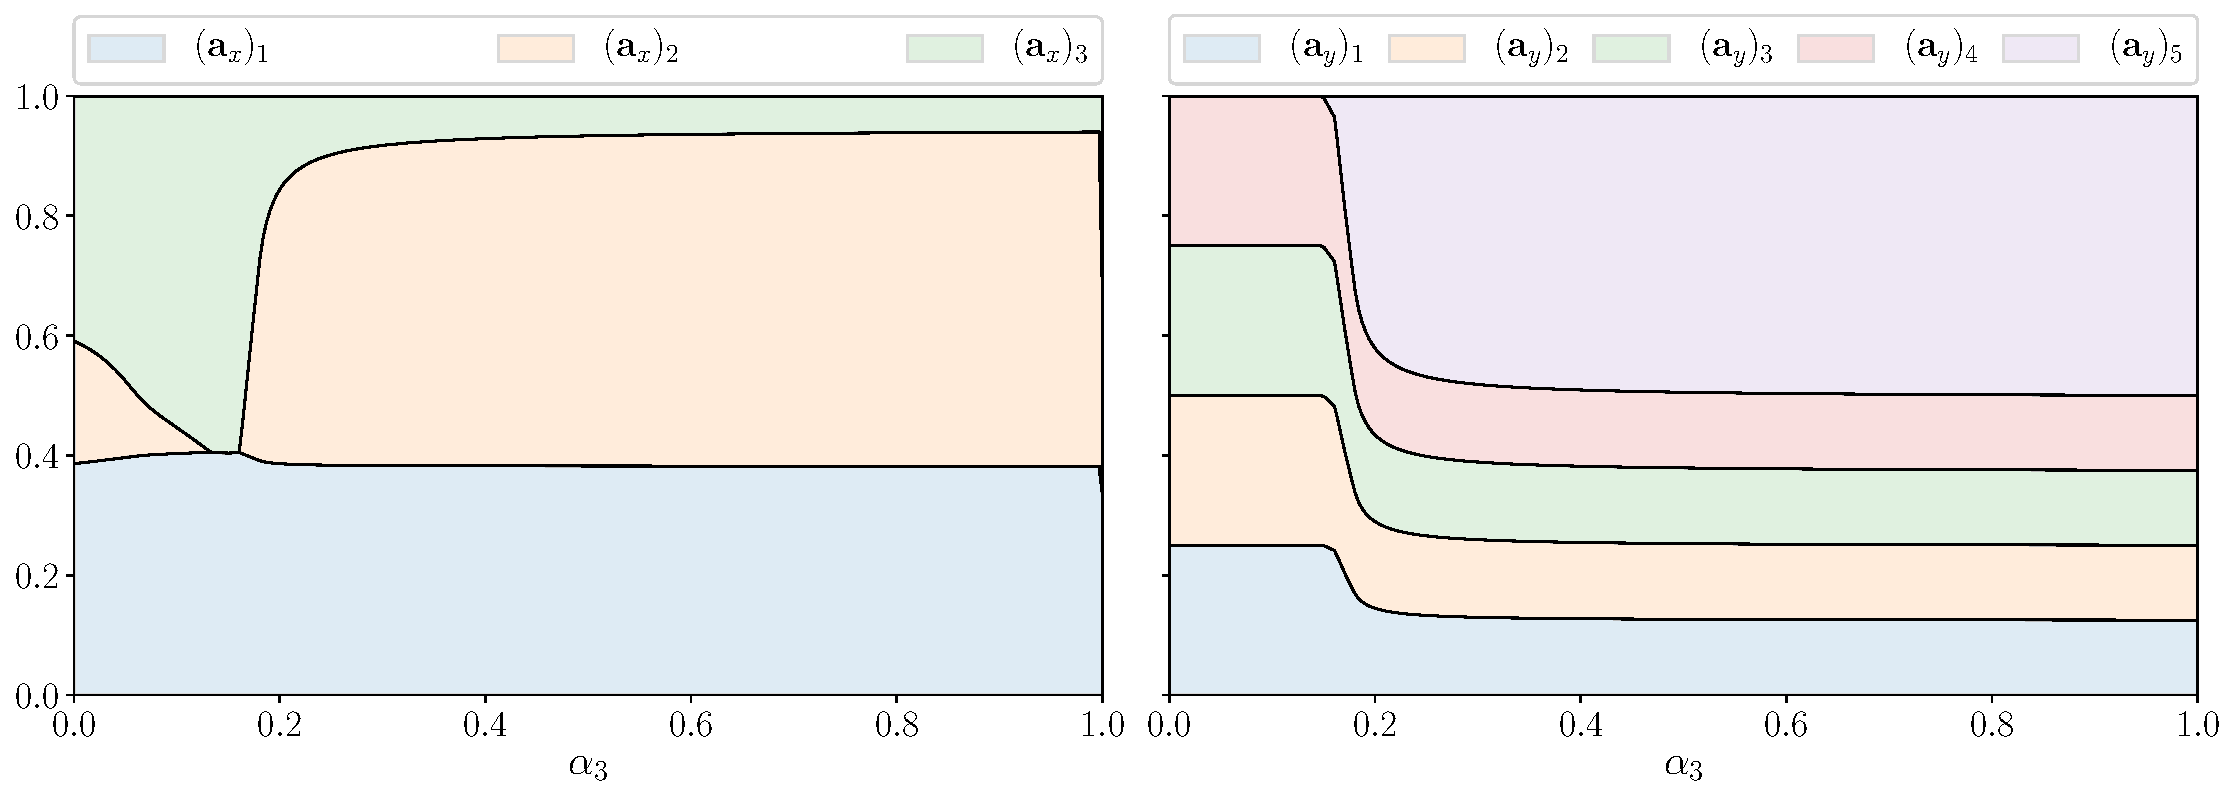
\includegraphics[width=\linewidth]{figs/features_vs_alpha.pdf}
	\caption{Feature importances $\ba_x$ and $\ba_y$ with respect to the $\alpha_3$ coefficient}
	\label{fig:features_vs_alpha}
\end{figure}

\paragraph{Minimax QPFS}
The functional~\eqref{eq:multivariate_quadratic_problem} is symmetric with respect to~$\ba_x$ and $\ba_y$. 
It penalizes features that are correlated and do not relevant to targets. 
At the same time it penalizes targets that are correlated and are not sufficiently explained by the features. 
It leads to small importances for targets which are difficult to predict by features and large importances for targets which are strongly correlated with features. 
It contradicts with the intuition. 
Our goal is to predict all targets, especially which are difficult to explain, by selected relevant and non-correlated features. We express this into two related problems. 
\begin{align}
	\alpha_1 \cdot \underbrace{\ba_x^T \bQ_x \ba_x}_{\text{Sim}(\bX)} - \alpha_2 \cdot \underbrace{\vphantom{()} \ba_x^T\mathbf{B} \ba_y}_{\text{Rel}(\bX, \bY)} \rightarrow \min_{\substack{\ba_x \geq \bZero_n, \\ \bOne_n^T\ba_x=1}}; 
	\label{eq:x_qpfs}\\
	\alpha_3 \cdot \underbrace{\ba_y^T \bQ_y \ba_y}_{\text{Sim}(\bY)} + \alpha_2 \cdot \underbrace{\vphantom{()} \ba_x^T \mathbf{B} \ba_y}_{\text{Rel}(\bX, \bY)} \rightarrow \min_{\substack{\ba_y \geq \bZero_r,  \\ \bOne_r^T\ba_y=1}}.
	\label{eq:y_qpfs}
\end{align}
The difference in Rel part.
In feature space the non-relevant components should have smaller scores. 
Meanwhile, the targets that are not relevant to the features should have larger scores.
The problems~\eqref{eq:x_qpfs} and \eqref{eq:y_qpfs} are merged into the joint min-max or max-min formulation
\begin{equation}
	\min_{\substack{\ba_x \geq \bZero_n \\ \bOne_n^T\ba_x=1}} 	\max_{\substack{\ba_y \geq \bZero_r \\ \bOne_r^T\ba_y=1}} f(\ba_x, \ba_y), \quad \left(\text {or} \, \max_{\substack{\ba_y \geq \bZero_r \\ \bOne_r^T\ba_y=1}} \min_{\substack{\ba_x \geq \bZero_n \\ \bOne_n^T\ba_x=1}} f(\ba_x, \ba_y)\right),
	\label{eq:minmax}
\end{equation}
where
\[
	f(\ba_x, \ba_y) = \alpha_1 \cdot \underbrace{\ba_x^T \bQ_x \ba_x}_{\text{Sim}(\bX)} - \alpha_2 \cdot \underbrace{\ba_x^T \bB \ba_y}_{\text{Rel}(\bX, \bY)} - \alpha_3 \cdot \underbrace{\ba_y^T \bQ_y \ba_y}_{\text{Sim}(\bY)}.
\]
The link between feature selection quality criteria~\eqref{eq:subset_selection} and the min-max problem~\eqref{eq:minmax} is the following
\begin{equation}
\cA = \argmax_{\cA' \subseteq \{1, \dots, n\}} Q(\cA' | \bX, \bY) \Leftrightarrow \argmin_{\ba_x \geq \bZero_n, \, \bOne_n^T\ba_x=1} \left[\max_{\substack{\ba_y \geq \bZero_r \\ \bOne_r^T\ba_y=1}} f(\ba_x, \ba_y)\right].
\end{equation}
\begin{theorem}
	For positive definite matrices $\bQ_x$ and $\bQ_y$ the max-min and min-max problems~\eqref{eq:minmax} have the same optimal value. 
\end{theorem}
\begin{proof}
	Denote 
	\begin{equation*}
	\mathbb{C}^n = \{\ba : \ba \geq \bZero_n, \, \bOne_n^T\ba=1\}, \quad \mathbb{C}^r = \{\ba : \ba \geq \bZero_r, \, \bOne_r^T\ba=1\};
	\end{equation*}
	The sets $\mathbb{C}^n$ and $\mathbb{C}^r$ are compact and convex. The function $f: \mathbb{C}^n \times \mathbb{C}^r \rightarrow \bbR$ is a continuous function. If $\bQ_x$ and $\bQ_y$ are positive definite matrices, the function~$f$ is convex-concave, i.e.
	$f(\cdot, \ba_y): \mathbb{C}^n \rightarrow \bbR$ is convex for fixed~$\ba_y$, and $f(\ba_x, \cdot): \mathbb{C}^r \rightarrow \bbR$ is concave for fixed~$\ba_x$. 
	In this case Neumann's minimax theorem states
	\[
	\min_{\ba_x \in \mathbb{C}^n} \max_{\ba_y \in \mathbb{C}^r} f(\ba_x, \ba_y) = \max_{\ba_y \in \mathbb{C}^r} \min_{\ba_x\in \mathbb{C}^n} f(\ba_x, \ba_y).
	\]
\end{proof}

To solve the min-max problem~\eqref{eq:minmax}, fix some~$\ba_x \in \mathbb{C}^n$. For fixed vector~$\ba_x$ we solve the problem
\begin{equation}
	\max_{\ba_y \in \mathbb{C}_r} f(\ba_x, \ba_y) = \max_{\substack{\ba_y \geq \bZero_r \\ \bOne_r^T\ba_y=1}} \bigl[\alpha_1 \cdot \ba_x^T \bQ_x \ba_x - \alpha_2 \cdot \ba_x^T \bB \ba_y - \alpha_3 \cdot \ba_y^T \bQ_y \ba_y \bigr].
	\label{eq:fixed_ax}
\end{equation}
The Lagrangian for this problem is
\[
	L(\ba_x, \ba_y, \lambda, \bmu) = \alpha_1 \cdot \ba_x^T \bQ_x \ba_x - \alpha_2 \cdot \ba_x^T \bB \ba_y - \alpha_3 \cdot \ba_y^T \bQ_y \ba_y + \lambda \cdot  (\bOne_r^T \ba_y - 1) + \bmu^T \ba_y.
\]
Here the Lagrange multipliers $\bmu$, corresponding to the inequality constraints $\ba_y \geq \bZero_r$, are restricted to be nonnegative. 
The dual problem is
\begin{equation}
	\min_{\lambda, \, \bmu \geq \bZero_r} g(\ba_x, \lambda, \bmu) = \min_{\lambda, \, \bmu \geq \bZero_r}  \left[\max_{\ba_y \in \bbR^r} L(\ba_x, \ba_y, \lambda, \bmu) \right].
	\label{eq:dual}
\end{equation}
The strong duality holds for the problem~\eqref{eq:fixed_ax}. Therefore, the optimal value for~\eqref{eq:fixed_ax} equals the optimal value for~\eqref{eq:dual}. It allows to solve the problem
\begin{equation}
	\min_{\ba_x \in \mathbb{C}^n, \, \lambda, \, \bmu \geq \bZero_r} g(\ba_y, \lambda, \bmu)
	\label{eq:dual_maxmin}
\end{equation}
instead of~\eqref{eq:minmax}.

Setting the gradient of the Langrangian $\nabla_{\ba_y} L(\ba_x, \ba_y, \lambda, \bmu)$ to zero, we obtain an optimal value~$\ba_y$:
\begin{equation}
	\ba_y = \frac{1}{2\alpha_3} \bQ_y^{-1} \left( - \alpha_2 \cdot \bB^T \ba_x +\lambda \cdot \bOne_r + \bmu \right).
	\label{eq:ax}
\end{equation}
The dual function is equal to
\begin{multline}
	g(\ba_x, \lambda, \bmu) 
	= \max_{\ba_y \in \bbR^r} L(\ba_x, \ba_y, \lambda, \bmu) = 
	\ba_x^T \left( - \frac{\alpha_2^2}{4\alpha_3} \bB \bQ_y^{-1} \bB^T - \alpha_1 \cdot \bQ_x\right) \ba_x \\ - \frac{1}{4 \alpha_3} \lambda^2 \cdot \bOne_r^T \bQ_y^{-1} \bOne_r - \frac{1}{4 \alpha_3} \bmu^T \bQ_y^{-1} \bmu + \frac{\alpha_2}{2 \alpha_3} \lambda \cdot \bOne_r^T \bQ_y^{-1} \bB^T \ba_x \\ - \frac{1}{2 \alpha_3} \lambda \cdot \bOne_r^T \bQ_y^{-1} \bmu + \frac{\alpha_2}{2 \alpha_3} \bmu^T \bQ_y^{-1} \bB^T \ba_x + \lambda. 
	 \label{eq:dual_quadratic_form}
\end{multline} 

It brings to the quadratic problem~\eqref{eq:dual_maxmin} with~$n + r + 1$ variables.

\paragraph{Minimax Relevances}

The problem~\eqref{eq:dual_maxmin} is not convex. If we shift the spectrum for the matrix of quadratic form~\eqref{eq:dual_quadratic_form}, the optimality is lost. To overcome this problem, we drop the term~$\text{Sim}(\bY)$. 

\begin{equation}
\min_{\substack{\ba_x \geq \bZero_n \\ \bOne_n^T\ba_x=1}} 	\max_{\substack{\ba_y \geq \bZero_r \\ \bOne_r^T\ba_y=1}} \left[ (1 - \alpha) \cdot \ba_x^T \bQ_x \ba_x - \alpha \cdot \ba_x^T \bB \ba_y \right],
\label{eq:minmax_rel}
\end{equation}
The Lagrangian for the problem~\eqref{eq:minmax_rel} with the fixed vector~$\ba_x$ is
\[
L(\ba_x, \ba_y, \lambda, \bmu) = (1 - \alpha) \cdot \ba_x^T \bQ_x \ba_x - \alpha \cdot \ba_x^T \bB \ba_y + \lambda \cdot  (\bOne_r^T \ba_y - 1) + \bmu^T \ba_y.
\]
Setting the gradient of the Langrangian $\nabla_{\ba_y} L(\ba_x, \ba_y, \lambda, \bmu)$ to zero, we obtain:
\begin{equation*}
\alpha \cdot \bB^T \ba_x = \lambda \cdot \bOne_r + \bmu.
\end{equation*}
The dual function is equal to
\begin{equation}
g(\ba_x, \lambda, \bmu) =
\begin{cases}
(1 - \alpha) \cdot \ba_x^T \bQ_x \ba_x - \lambda, & \alpha \cdot \bB^T \ba_x = \lambda \cdot \bOne_r + \bmu;  \\
+ \infty, & \text{otherwise}.
\end{cases}
\end{equation} 
In this case the feature scores is the solution of~\eqref{eq:dual_maxmin}. 

\begin{statement}
	For the case $r=1$ the proposed functionals~\eqref{eq:multivariate_quadratic_problem} and~\eqref{eq:minmax} coincide with the original QPFS algorithm~\eqref{eq:quadratic_problem}.
	
	\begin{proof}
		If $r$ is equal to 1, then $\bQ_y = q_y$ is a scalar, $\ba_y = 1$, $\bB = \bb$. It reduces the problems~\eqref{eq:multivariate_quadratic_problem} and~\eqref{eq:minmax} to 
		\[
		\alpha_1 \cdot \ba_x^T \bQ_x \ba_x - \alpha_2 \cdot \ba_x^T \bb \rightarrow \min_{\ba_x \geq \bZero_n, \, \bOne_n^T\ba_x=1} .
		\]
		Setting $\alpha = \frac{\alpha_2}{\alpha_1 + \alpha_2}$ brings to the original QPFS problem~\eqref{eq:quadratic_problem}.
	\end{proof}
\end{statement}

\section{Feature categorization}
Feature selection algorithms eliminate features which are not relevant to the target variable. 
To determine whether the feature is relevant the t-test could be applied for the correlation coefficient.
\[
	r = \text{corr} (\bchi, \bnu), \quad t = \frac{r \sqrt{m - 2}}{1 - r^2} \sim \text{St} (m - 2).
\]
\begin{align*}
&H_0: r = 0 \\
&H_1: r \neq 0
\end{align*}
If features are relevant, but correlated, feature selection methods pick the subset of them to reduce the multicollinearity and redundancy.
The goal is to find relevant, non-correlated features. 
However, in this case the correlations between targets in matrix~$\bY$ are crucial.
To measure the dependence of each feature or target, the Variance Inflation Factor (VIF) is computed
\[
	\text{VIF}(\bchi_j) = \frac{1}{1 - R_j^2}, \quad \text{VIF}(\bnu_k) = \frac{1}{1 - R_k^2},
\]
where $R_j^2$($R_k^2$) are coefficients of determination for the regression of $\bchi_j$($\bnu_k$) on the other features(targets).

On that basis, we categorize features into 5 disjoint groups:
\begin{enumerate}
	\item non-relevant features
	\[
		\left\{j: \text{corr}(\bchi_j, \bnu_k) = 0, \, \forall k \in \{1, \dots, r\}\right\};
	\]
	\item non-$\bX$-correlated features, which are relevant to non-$\bY$-correlated targets
	\[
		\left\{j: \left(\text{VIF}(\bchi_j) < 10\right) \, \text{and} \, \left(\text{VIF}(\bnu_k) < 10 , \, \forall k \in \{1, \dots, r\}: \,  \text{corr}(\bchi_j, \bnu_k) \neq 0 \right)\right\};
	\]
	\item non-$\bX$-correlated features, which are relevant to $\bY$-correlated targets
	\[
		\left\{j: \left(\text{VIF}(\bchi_j) < 10\right) \, \text{and} \, \left( \exists k \in \{1, \dots, r\}: \text{VIF}(\bnu_k) > 10 \,\, \& \,\, \text{corr}(\bchi_j, \bnu_k) \neq 0 \right)\right\};
	\]
	\item $\bX$-correlated features, which are relevant to non-$\bY$-correlated targets
	\[
		\left\{j: \left(\text{VIF}(\bchi_j) > 10\right) \, \text{and} \, \left(\text{VIF}(\bnu_k) < 10 , \, \forall k \in \{1, \dots, r\}: \,  \text{corr}(\bchi_j, \bnu_k) \neq 0 \right)\right\};
	\]
	\item $\bX$-correlated features, which are relevant to $\bY$-correlated targets
	\[
		\left\{j: \left(\text{VIF}(\bchi_j) > 10\right) \, \text{and} \, \left( \exists k \in \{1, \dots, r\}: \text{VIF}(\bnu_k) > 10 \,\, \& \,\, \text{corr}(\bchi_j, \bnu_k) \neq 0 \right)\right\}.
	\]
\end{enumerate}

%%%%%%%%%%%%%%%%%%%%%%%%%%%%%%%%%%%%%%%%%%%%%%%%
\section{Metrics}
%%%%%%%%%%%%%%%%%%%%%%%%%%%%%%%%%%%%%%%%%%%%%%%%

To evaluate the selected subset~$\cA$ we introduce criteria that estimate the quality of feature selection procedure. 
Variance Inflation Factor is the measure of multicollinearity in the matrix. We take the maximum VIF across all matrix columns:  
\[
	\text{VIF} = \max_{j \in \cA} \text{VIF} (\bchi_j).
\]
The model stability is given by the logarithm of the ratio between minimal~$\lambda_{\min}$ and maximum~$\lambda_{\max}$ eigenvalue of the matrix~$\bX^T \bX$:
\[
	R = \ln \frac{\lambda_{\min}}{\lambda_{\max}}.
\]
The Root Mean Squared Error (RMSE) shows the quality of the model prediction. We estimate RMSE at the train and test data.
\[
	\text{RMSE}(\bY, \widehat{\bY}_{\cA}) = \sqrt{\text{MSE} (\bY, \widehat{\bY}_{\cA})} =  \| \bY - \widehat{\bY}_{\cA} \|_2, \quad \text{where} \quad \widehat{\bY}_{\cA} = \bX_{\cA} \bTheta_{\cA}^T.
\]
Akaike Information Criteria (AIC) is a trade-off between prediction quality and the size of selected subset~$\cA$:
\[
	\text{AIC} = m \ln \left( \frac{\text{MSE} ( \bY, \widehat{\bY}_{\cA})}{m}\right) + 2 | \cA |.
\]

%%%%%%%%%%%%%%%%%%%%%%%%%%%%%%%%%%%%%%%%%%%%%%%%
\section{Experiment}
%%%%%%%%%%%%%%%%%%%%%%%%%%%%%%%%%%%%%%%%%%%%%%%%
We carried out computational experiment with ECoG data from the NeuroTycho project. The input data consists of brain voltage signals recorded from 32 channels. 
The goal is to predict 3D hand position in the next moments given the input signal. 
The example of input signals and the 3D wrist coordinates are shown in Figure~\ref{fig:ecog_data}. 
The initial voltage signals are transformed to the spatial-temporal representation using wavelet transformation. 
The procedure of extracting feature representation from the raw data are described in details in~[links]. 
Feature description in each time moment has dimension equals to 32 (channels) $\times$ 27 (frequencies) = 864. 
Each object is the representation of local history time segment with duration $\Delta t = 1s$. The time step between objects is $\delta t =  0.05s$. 
The final matrices are $\bX \in \bbR^{18900 \times 864}$ and $\bY \in \bbR^{18900 \times 3k}$, where $k$ is a number of moments that we predict. 
We split our data into train and test parts with the ratio 0.67.

\begin{figure}
	\centering
	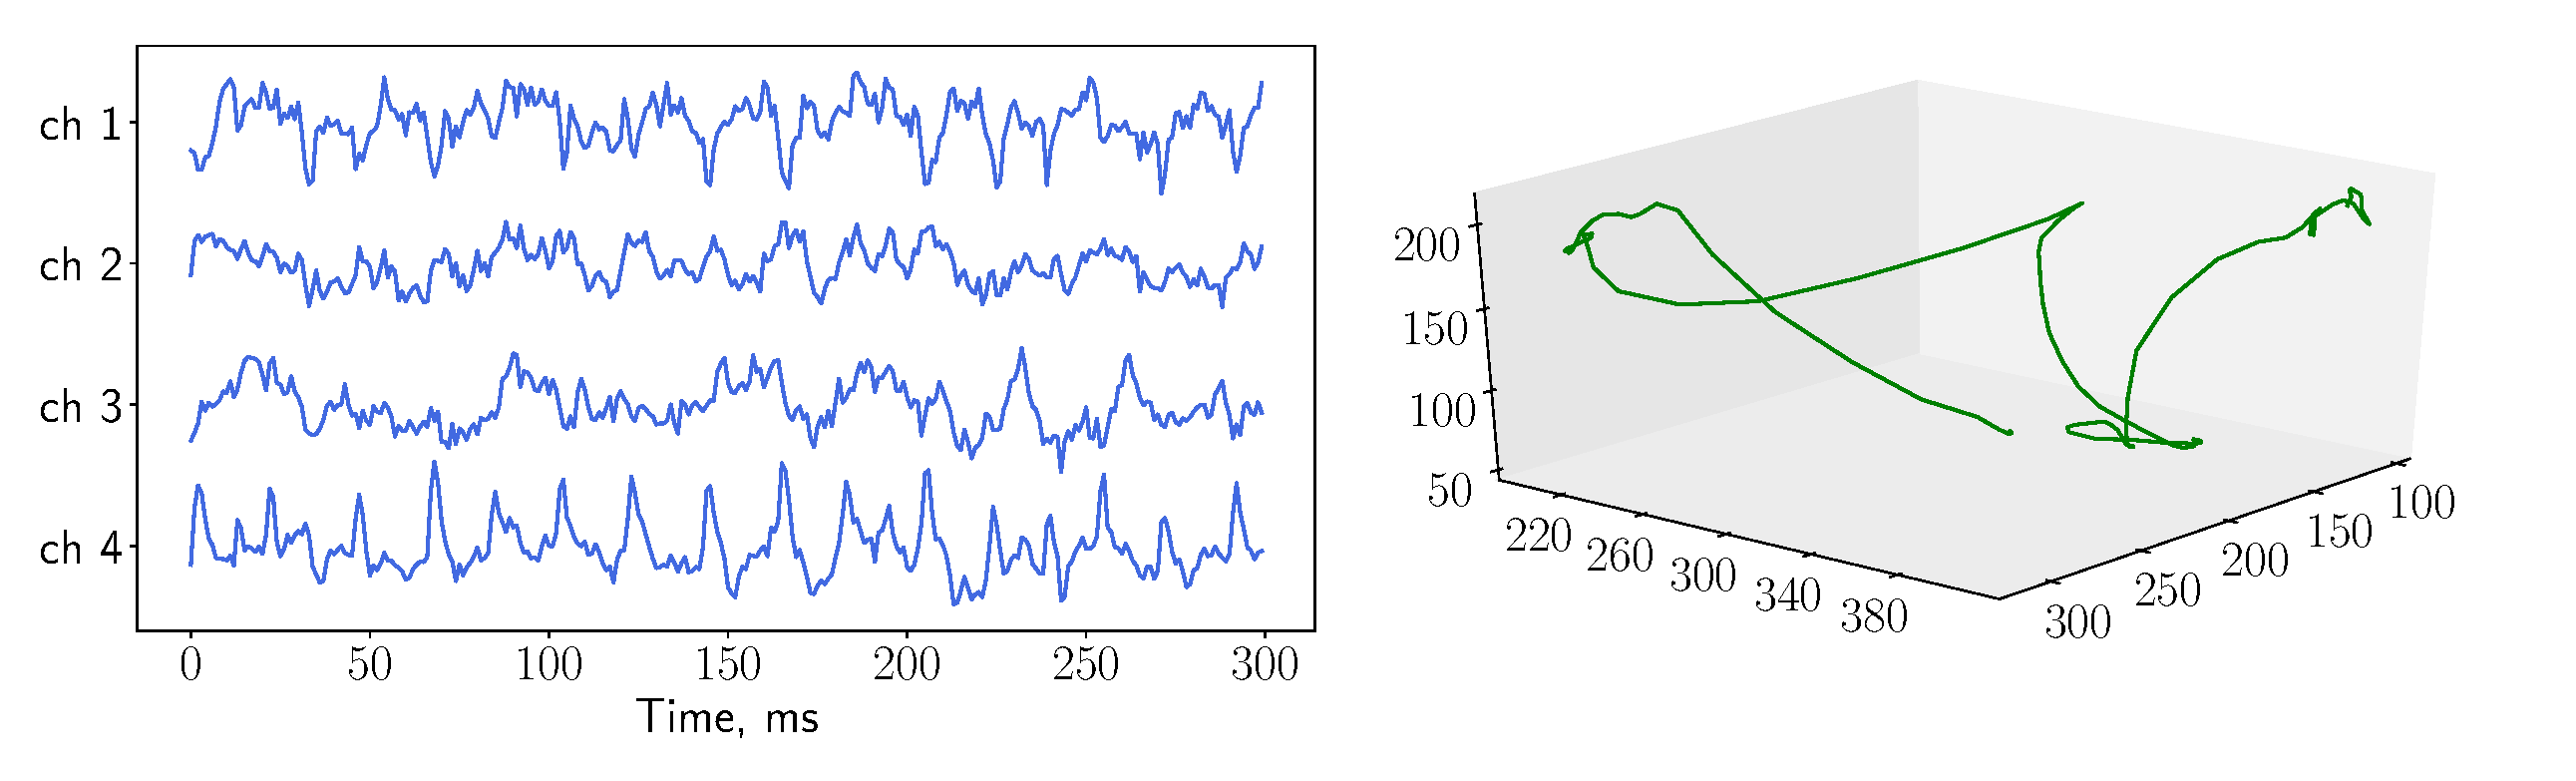
\includegraphics[width=\linewidth]{figs/ecog_data}
	\caption{Brain signals and the corresponding hand position}
	\label{fig:ecog_data}
\end{figure} 

Figures~\ref{fig:feature_scores_ex} and~\ref{fig:train_test_qpfs} show the result of the QPFS algorithm, where we use the Relevance Aggregation strategy and $k = 1$. 
QPFS scores~$\ba_x$ decrease sharply. 
Only about one hundred features have scores significantly greater that zero. 
The test error stops to decrease using this one hundred features. 
It confirms that the initial data representation is redundant.   
\begin{figure}
	\begin{minipage}{.5\linewidth}
		\centering
		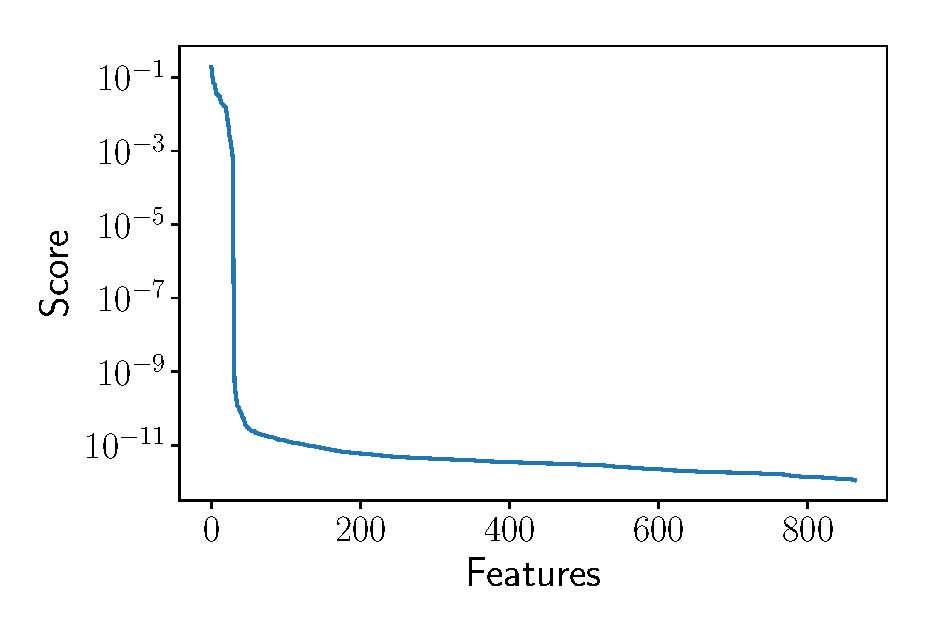
\includegraphics[width=\linewidth]{figs/feature_scores_ex.eps}
		\caption{Sorted feature importances for \\ the QPFS algorithm}
		\label{fig:feature_scores_ex}
	\end{minipage}%
	\begin{minipage}{.5\linewidth}
	\centering
	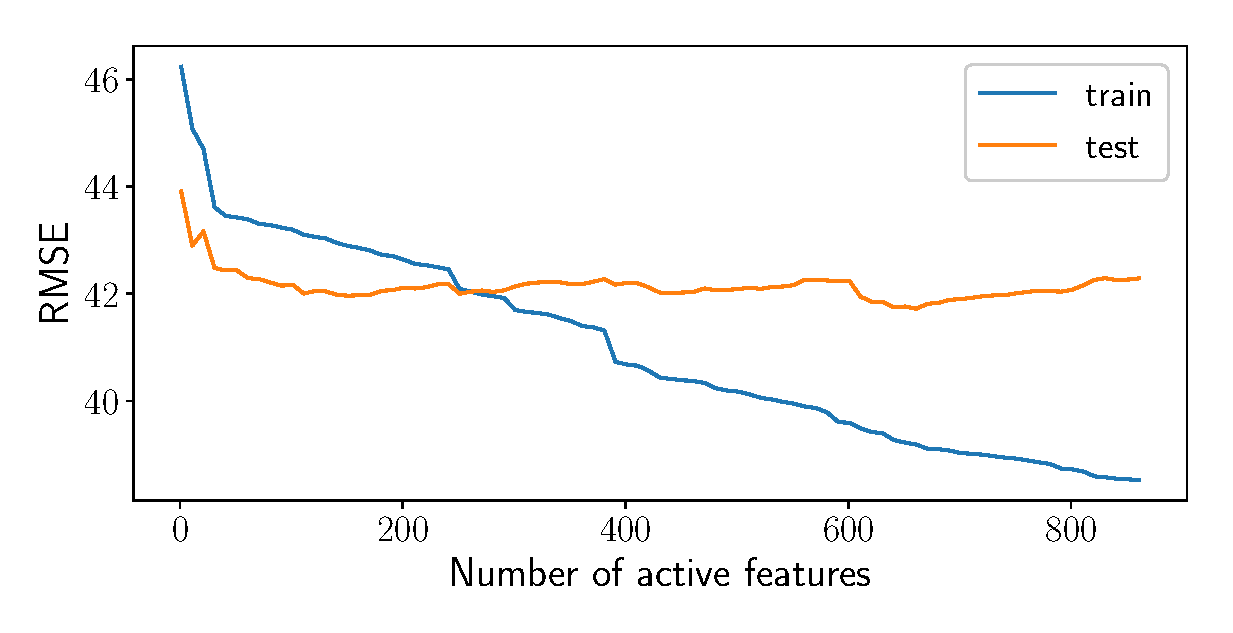
\includegraphics[width=\linewidth]{figs/train_test_qpfs.eps}
	\caption{RMSE w.r.t. size of active set, features are ranked by QPFS algorithm}
	\label{fig:train_test_qpfs}
	\end{minipage}
\end{figure}

Figure~\ref{fig:corr_matrix} shows the dependencies in the matrices~$\bX$ and~$\bY$. Some frequencies in the matrix~$\bX$ are highly correlated. 
The correlations between axes are not significant in comparison with correlations between consequent moments.
\begin{figure}
	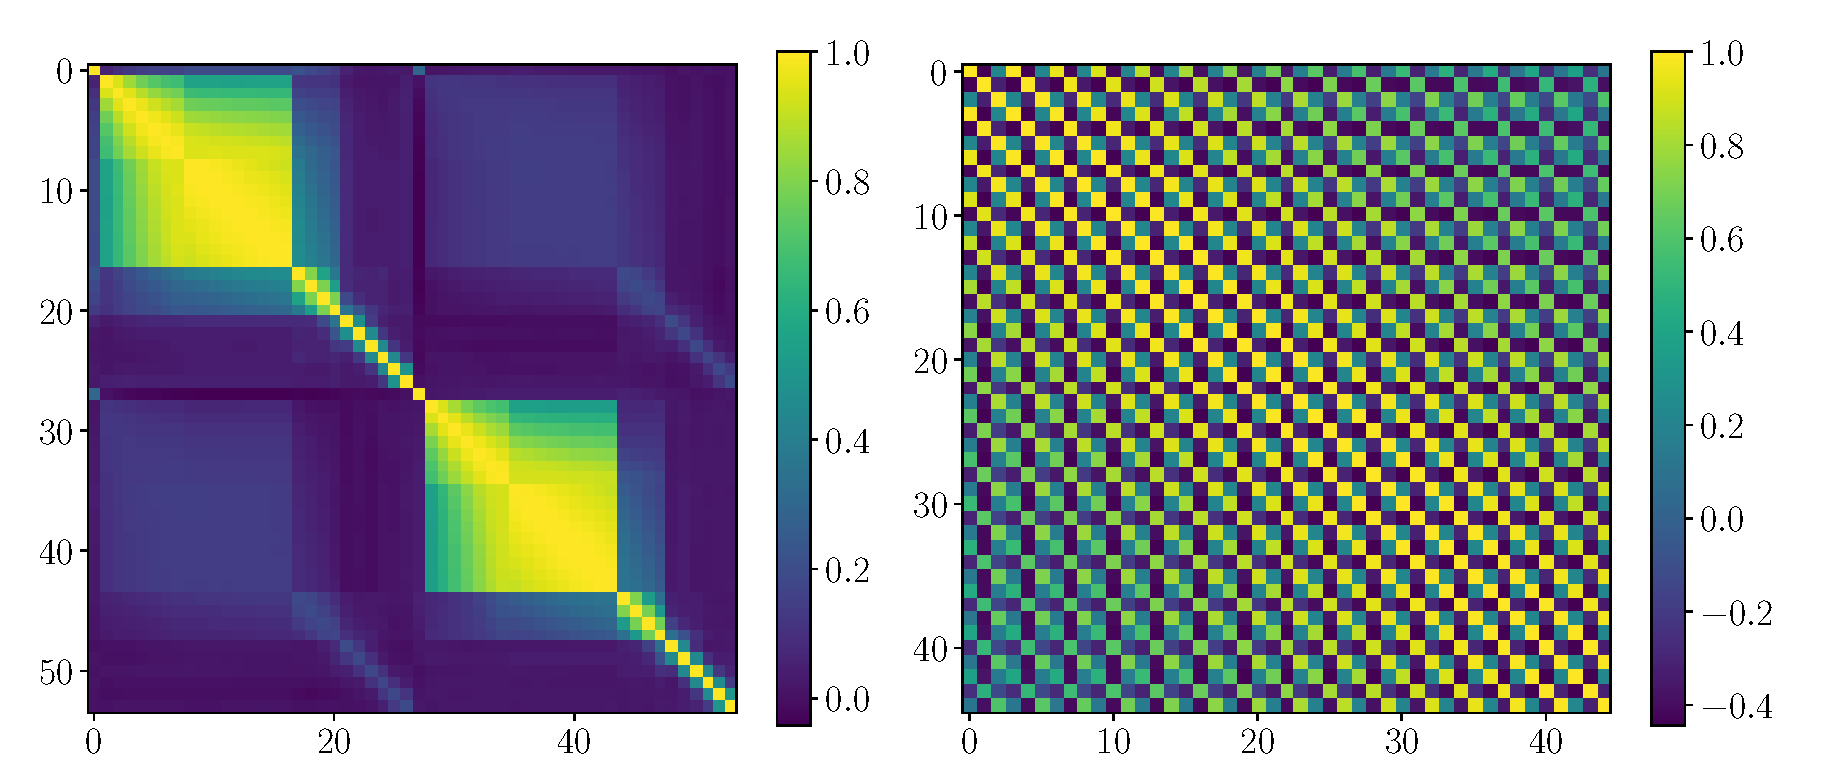
\includegraphics[width=\linewidth]{figs/corr_matrix.eps}
	\caption{Correlation matrices for $\bX$ and $\bY$}
	\label{fig:corr_matrix}
\end{figure}

We apply QPFS algorithm with Relevance Aggregation strategy for different values of~$\alpha_3$ coefficient according to formulas~\eqref{eq:alphas3}. 
The dependence between target scores~$\ba_y$ with respect to~$\alpha_3$ for different values of~$k$ are shown in Figure~\ref{fig:features_vs_alpha_ecog}. 
If we predict wrist coordinates only for one moment $k = 1$ targets scores are almost the same. 
It tells about the independence between $x$, $y$, and $z$ coordinates. 
For $k = 2$ and $k = 3$ the scores of some targets becomes zero when $\alpha_3$ increase. 

\begin{figure}
	\begin{minipage}{.5\linewidth}
		\subfloat[k=1]{\label{fig:autoreg_step1}
			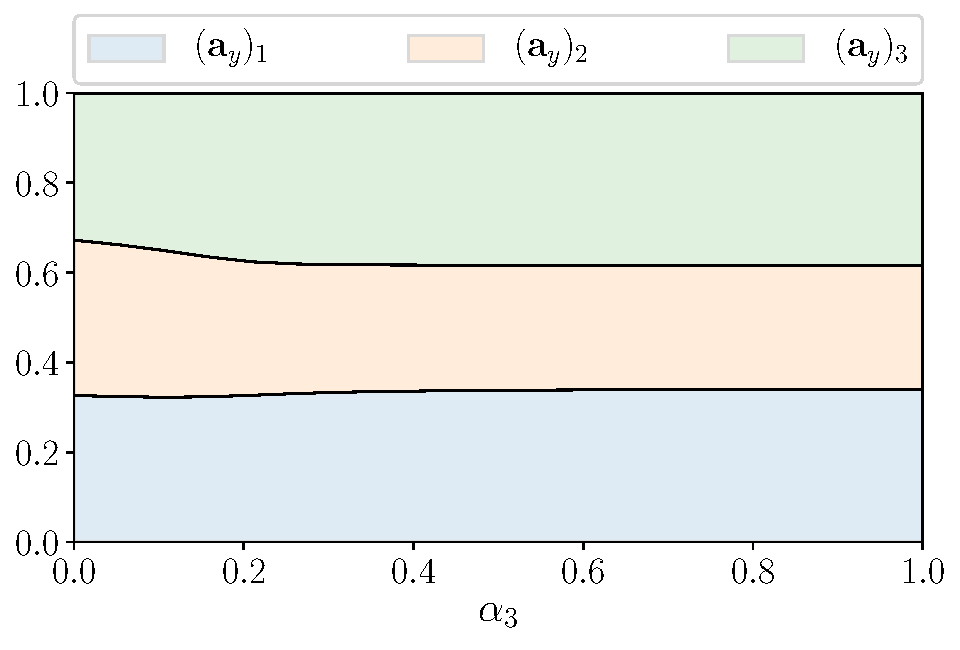
\includegraphics[width=\linewidth]{figs/features_vs_alpha_ecog_3.pdf}}
	\end{minipage}%
	\begin{minipage}{.5\linewidth}
		\subfloat[k=2]{\label{fig:autoreg_step2}
			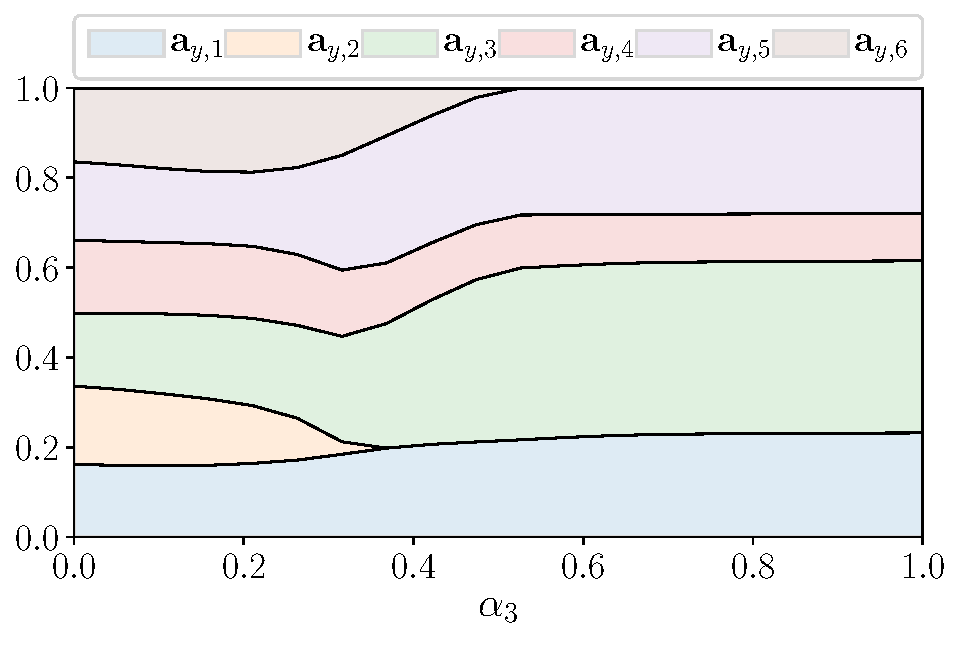
\includegraphics[width=\linewidth]{figs/features_vs_alpha_ecog_6.pdf}}
	\end{minipage}\par\medskip
	\subfloat[k=3]{\label{fig:autoreg_step3}
		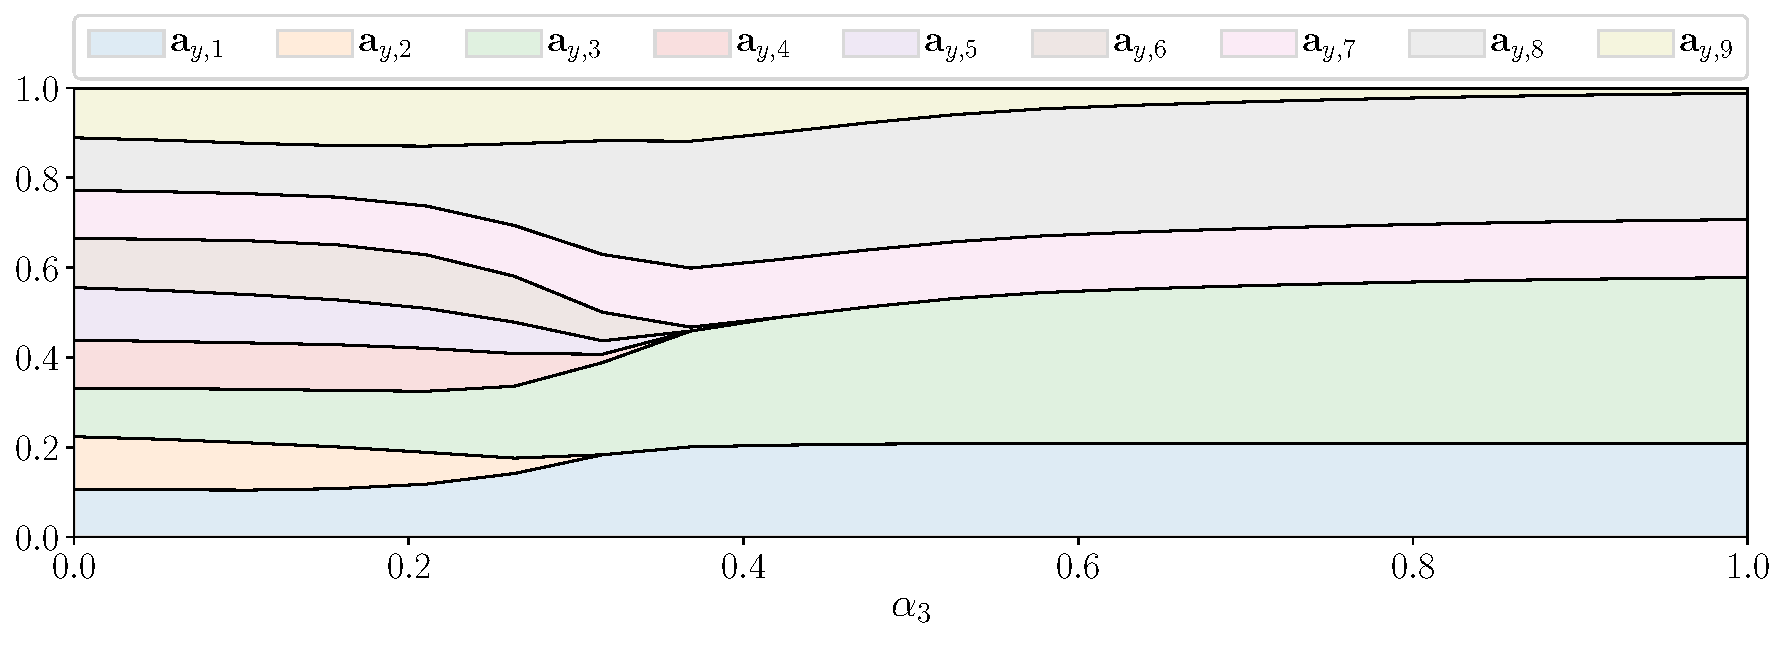
\includegraphics[width=\linewidth]{figs/features_vs_alpha_ecog_9.pdf}}
	
	\caption{Target importances~$\ba_y$ with respect to~$\alpha_3$ for QPFS with Relevance Aggregation}
	\label{fig:features_vs_alpha_ecog}
\end{figure}

We compare the proposed strategies of multivariate QPFS for the ECoG dataset. 

\begin{figure}
	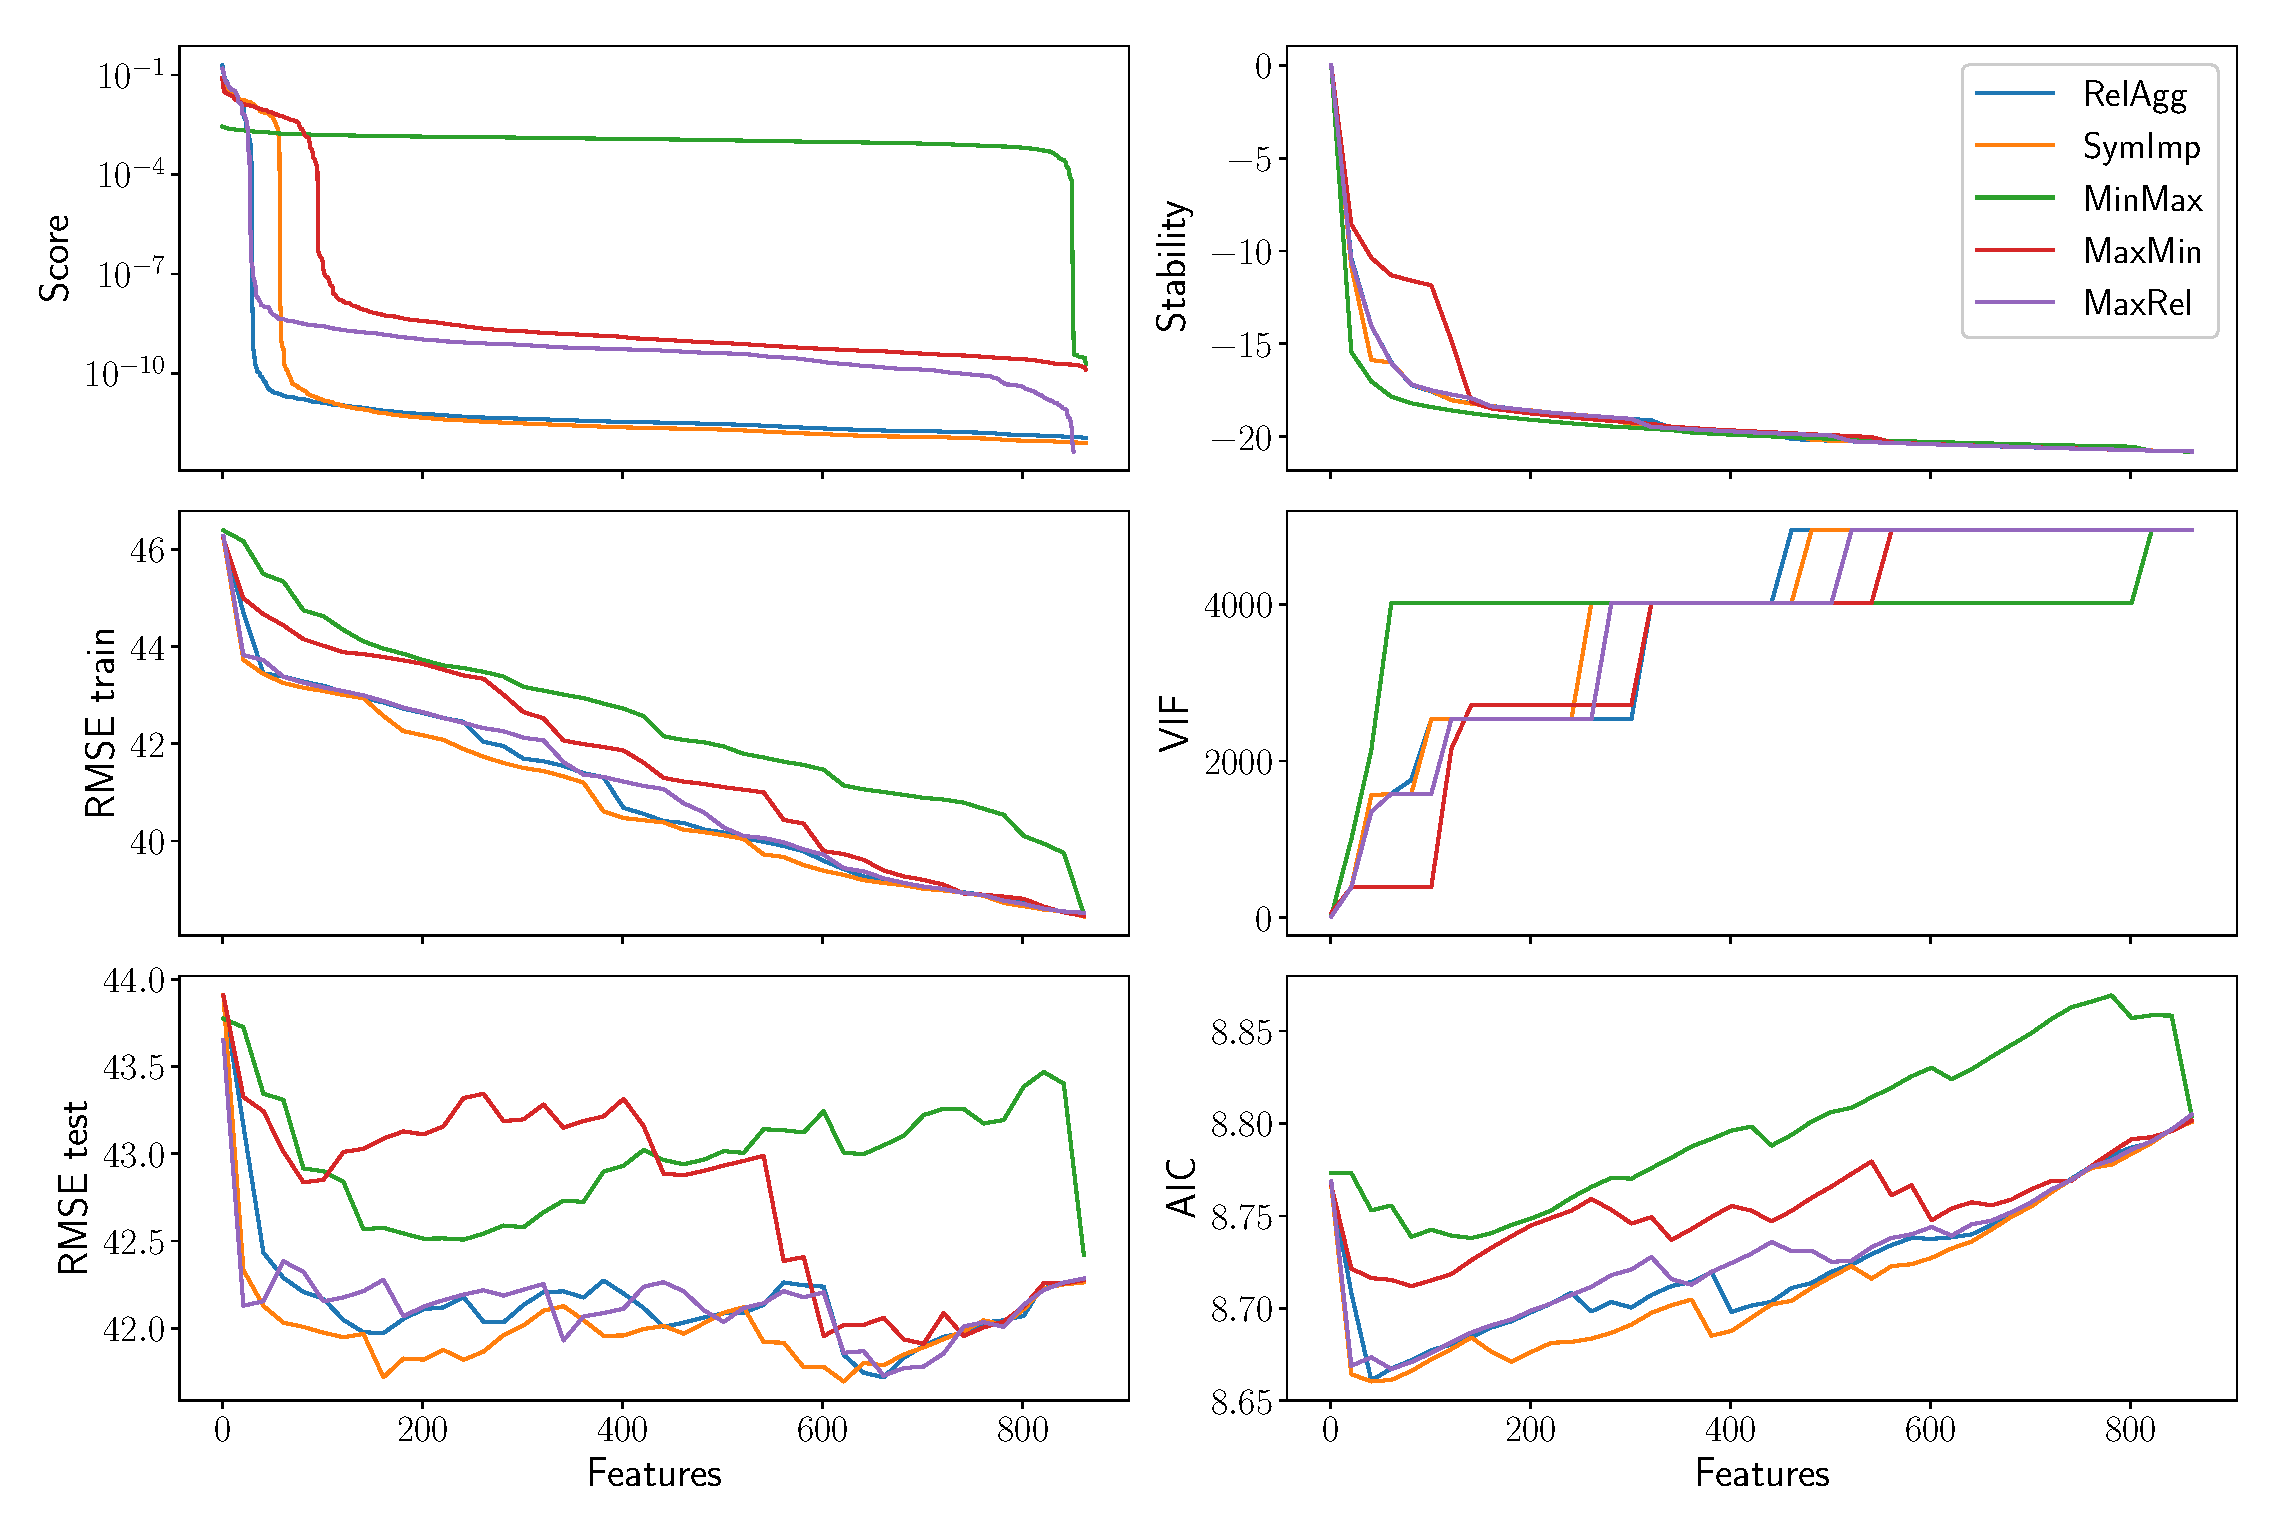
\includegraphics[width=\linewidth]{figs/ecog_3_1_metrics.eps}
	\caption{autoregression step = 1}
\end{figure}

\begin{figure}
	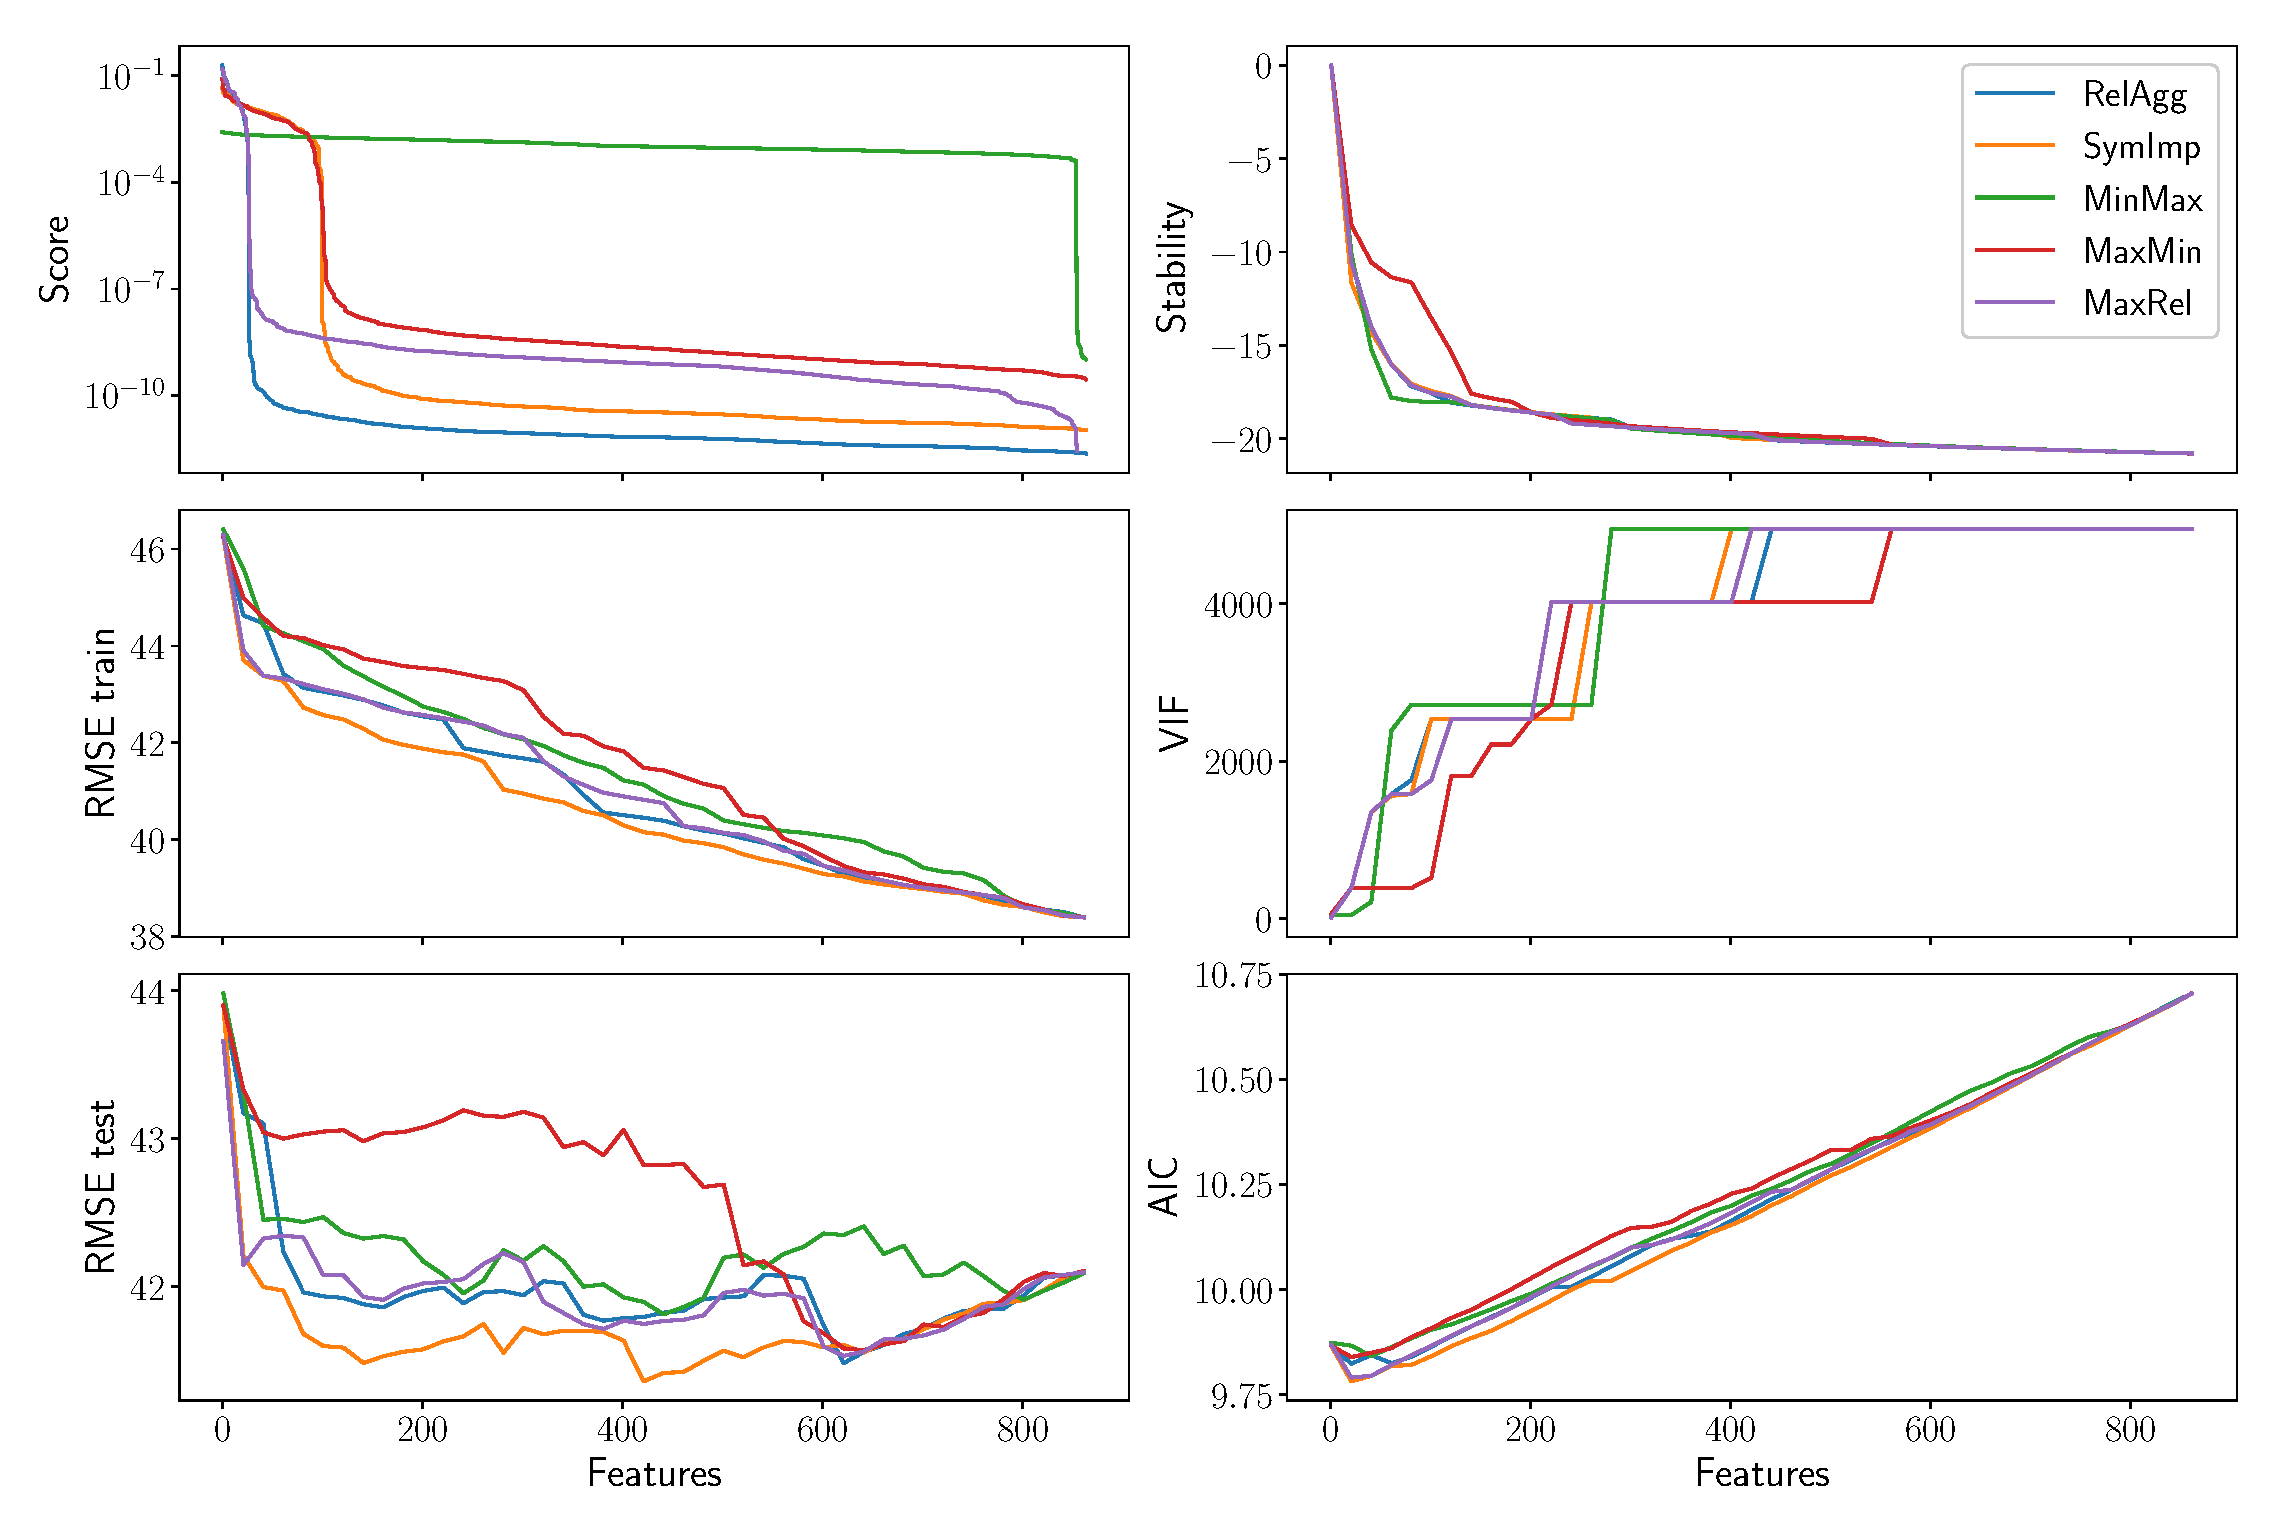
\includegraphics[width=\linewidth]{figs/ecog_3_3_metrics.eps}
	\caption{autoregression step = 3}
\end{figure}

\begin{figure}
	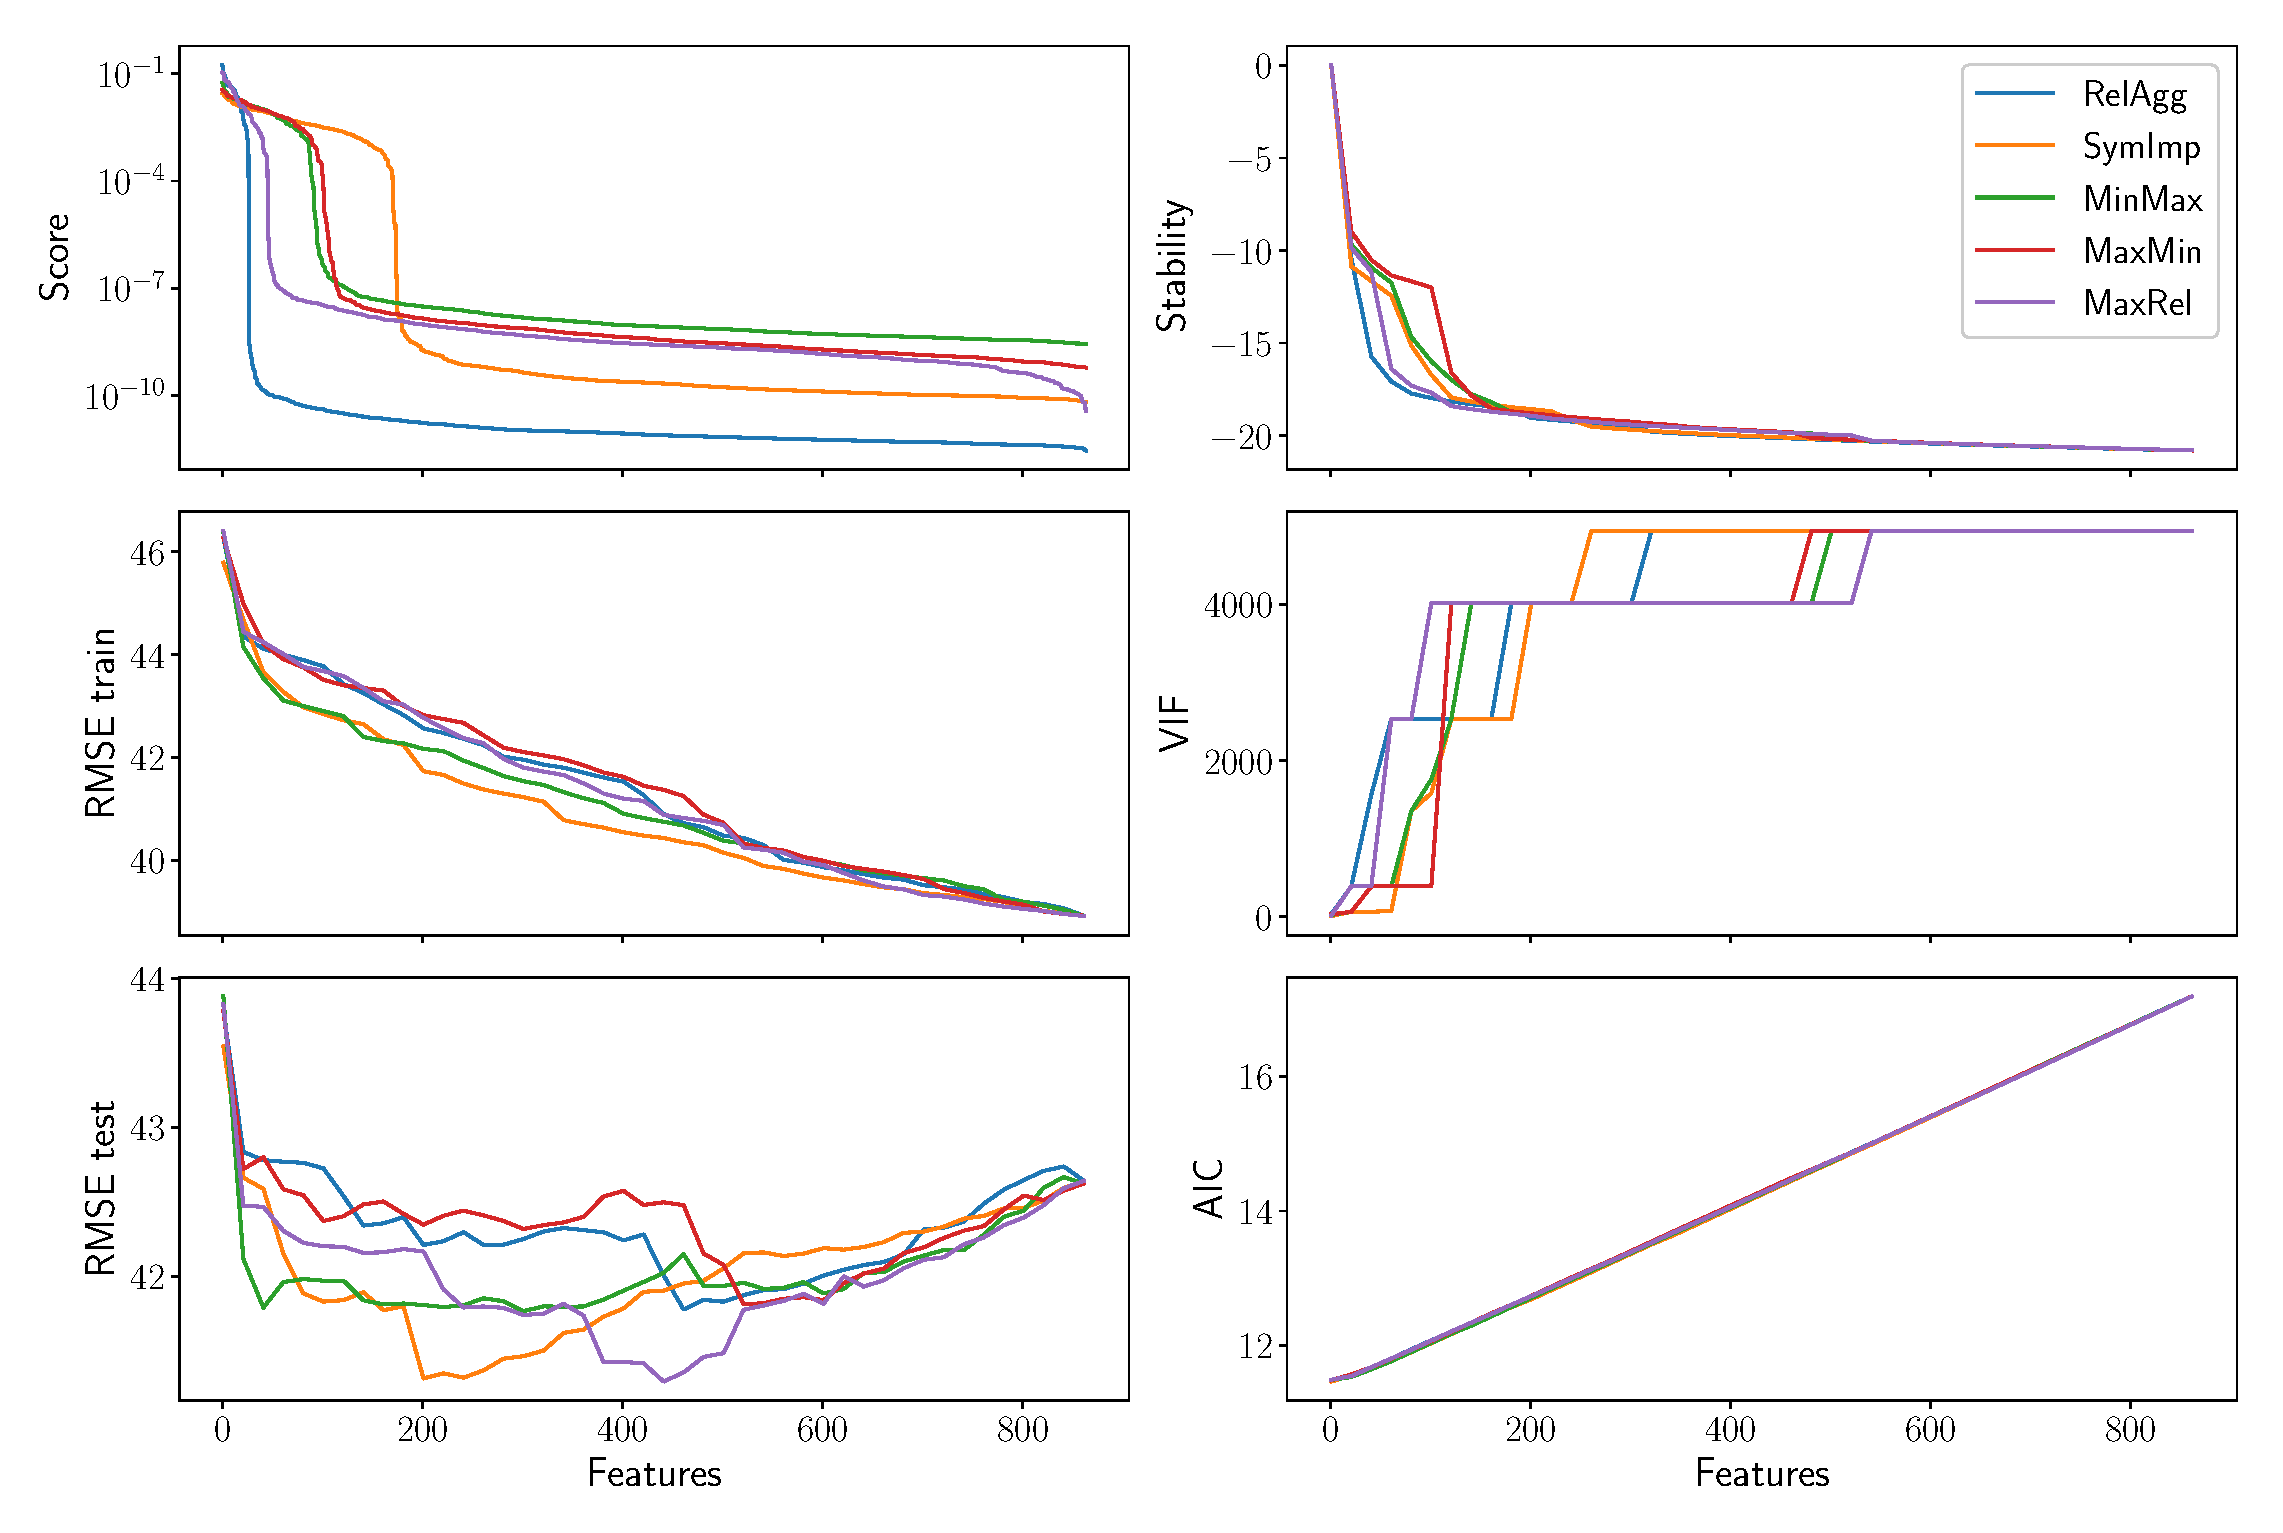
\includegraphics[width=\linewidth]{figs/ecog_3_15_metrics.eps}
	\caption{autoregression step = 15}
\end{figure}
\end{document}